%%=============================================================================
%% CAPITULO 3 -- PROCEDIMENTOS METODOLOGICOS
%%
%% Texto dummy (exercicio ia-6.1): trechos do pre-projeto do autor (versao 7).
%%=============================================================================

\section{Procedimentos metodológicos}

A estratégia metodológica incorpora princípios de Design Science Research,
especialmente a construção e avaliação de um artefato orientado a um problema
relevante. O artefato principal será o pipeline de geração e avaliação de dados
sintéticos, e não o modelo CTGAN isoladamente. Essa distinção é importante porque
o objeto de avaliação é o processo completo --- preparação, geração, validação e
uso analítico --- e não apenas o algoritmo.
% TODO: referência -- o pré-projeto cita Hevner et al. (2004) e Peffers et al.
% (2007) neste trecho; entram no .bib quando forem conferidas.

A preparação seguirá um fluxo de data airlock, representado na
Figura~\ref{fig:airlock}: (1) extração controlada; (2) identificação de
atributos sensíveis; (3) remoção ou transformação de identificadores; (4)
generalização ou agrupamento de categorias raras quando necessário; (5) criação
do dataset de treinamento; e (6) manutenção de um conjunto real de teste
isolado. O conjunto de teste real permanecerá inacessível ao treinamento do
gerador e será utilizado exclusivamente para avaliação final de utilidade.

\begin{figure}[htb]
  \caption{Fluxo de preparação dos dados (data airlock)}
  \label{fig:airlock}
  \centering
  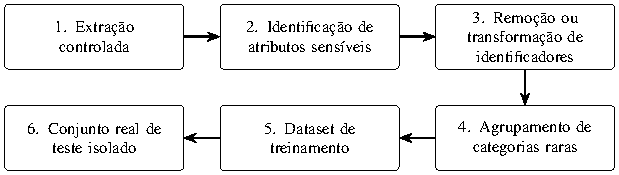
\includegraphics[width=\textwidth]{figuras/airlock.pdf}
  \fonte{Elaborado pelo autor (2026).}
\end{figure}

O pipeline metodológico será organizado em seis etapas: análise exploratória e
preparação dos dados; geração sintética com CTGAN e, quando viável, um baseline
não neural; avaliação de fidelidade; avaliação de utilidade analítica; avaliação
de risco de exposição; e síntese dos resultados e definição das condições de uso.
A Tabela~\ref{tab:avaliacao} relaciona as etapas de avaliação às técnicas de
análise e às hipóteses do estudo.

\begin{table}[htb]
  \caption{Etapas de avaliação, técnicas de análise e hipóteses}
  \label{tab:avaliacao}
  \centering
  \begin{tabular}{lll}
    \toprule
    \textbf{Etapa} & \textbf{Técnicas de análise} & \textbf{Hipótese} \\
    \midrule
    Fidelidade & Distribuições, KS, associações e clustering & H1 \\
    Utilidade  & TRTR $\times$ TSTR; PR-AUC, recall e F1     & H2 \\
    Exposição  & Proximidade, memorização e membership       & H3 \\
    \bottomrule
  \end{tabular}
  \fonte{Elaborado pelo autor (2026).}
\end{table}
